\documentclass{article}
%Paquete para agregar imagenes
\usepackage{graphicx}
%Paquete para usar la opcion H (posicion) en las imagenes
\usepackage{float}
%Ruta de las capturadas utilizadas
\graphicspath{ {capturas/tunelssh//} }

\title{Practica 3: Ataque ARP Spoofing y tunneling con SSH}
\author{Juan Carlos Perales de Jes\'us, Yafte Aaron Flores, Ra\'ul C\'astulo Ortega}
\date{19 Octubre 2017}
\
\makeindex

\begin{document}
\maketitle
\newpage

\section{Res\'umen}

\section{Introducci\'on}
Cuando un equipo pertenece a una red es posible que \'este pueda ver el tr\'afico de la red, si la navegaci\'on no es segura, dicho equipo puede ver en claro la informaci\'on que se env\'ia por la red.
 
\section{Objetivo}
\subsection{ARP Spoofing}
\subsection{Tunel SSH}
Cifrar un canal de comunicaci\'on para navegar por la red a\'un por sitios no seguros.

\section{Planteamiento del problema}
\subsection{ARP Spoofing}

\subsection{Tunel SSH}
Con herramientas de sniffering como Wireshark es posible ver el tr\'afico de la red, para evitar mandar paquetes con informaci\'on en claro, blindaremos el canal de comunicaci\'on.

\section{Metodolog\'ia a emplear}
\subsection{ARP Spoofing}

\subsection{Tunel SSH}
Crearemos un tunel SSH para redirigir el tr\'afico de la red a trav\'es de otra m\'aquina, el flujo de paquetes pasar\'a por un canal SSH, el cual es cifrado, \'esto evitar\'a enviar paquetes en claro por la red.

\section{Materiales}

\subsection{ARP Spoofing}
\begin{enumerate}
	\item 
\end{enumerate}

\subsection{Tunel SSH}
\begin{enumerate}
\item M\'aquina virtual con Kali-Linux
\item Sistema Operativo Windows \(7,8,10\)
\item Putty
\item OpenSSH
\item Wireshark
\item Navegador Web Firefox
\end{enumerate}

\section{Desarrollo}
\subsection{ARP Spoofing}

\subsection{Tunel SSH}
Los siguientes pasos se llevarón a cabo desde el sistema operativo Windows 10, con una m\'aquina virtual con Kali linux.

\subsubsection{Obtener IP de m\'aquina host (windows) y m\'aquina virtual (kali linux)}
En Windows abrimos la l\'inea de comandos de windows \emph{cmd} y tecleamos \emph{ipconfig}
En este caso la IP del host es \emph{192.168.0.102}

%Imagen 1
\begin{figure}[H]
\centering
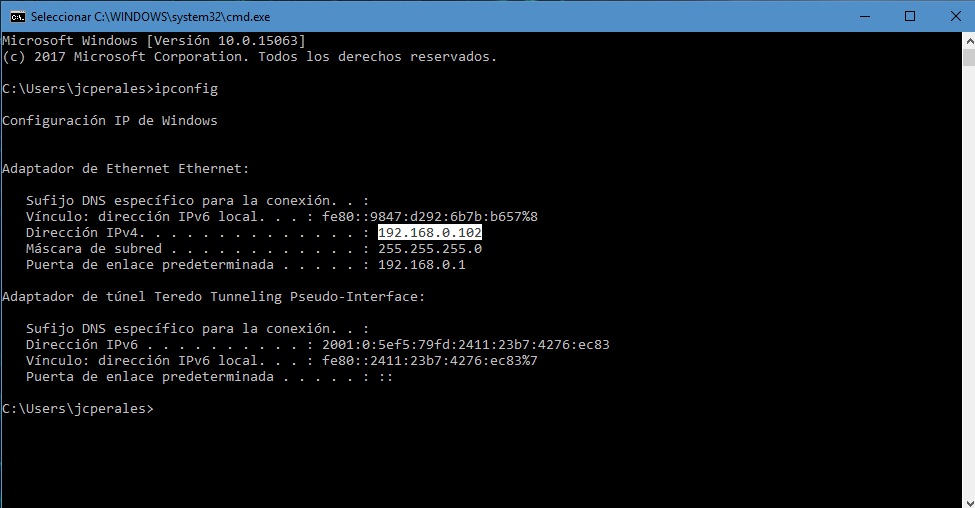
\includegraphics[width=1\textwidth]{01-IPCONFIG}
\end{figure}

En la m\'aquina virtual abrimos una terminal y ejecutamos el comando \emph{ifconfig}, la interfaz \emph{eth0} nos reporta la direcci\'on IP \emph{10.0.2.15}

%Imagen 2
\begin{figure}[H]
\centering
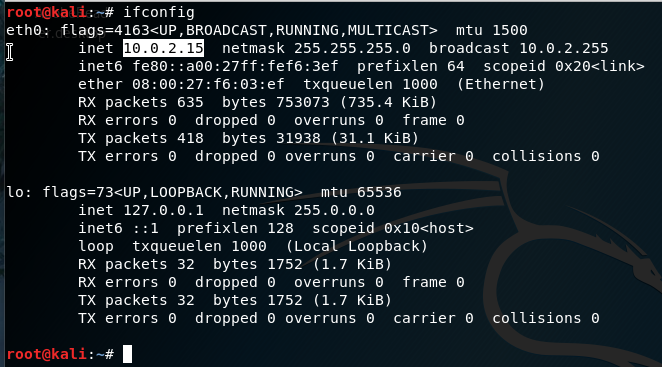
\includegraphics[width=1\textwidth]{02-IFCONFIG}
\end{figure}


\subsubsection{Configuraci\'on de VirtualBox}

Ya que conocemos ambas direcciones IP, en Virtualbox nos vamos a \emph{Dispositivos/Red/Preferencias de Red}

%Imagen 3
\begin{figure}[H]
\centering
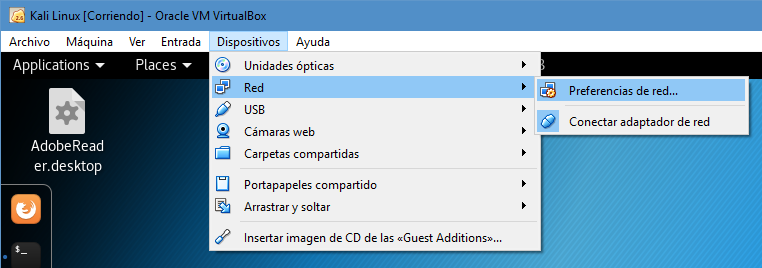
\includegraphics[width=1\textwidth]{03-PREFERENCIADERED}
\end{figure}

Desp\'ues damos clic en el bot\'on que dice \emph{Reenv\'io de Puertos}

%Imagen 4
\begin{figure}[H]
\centering
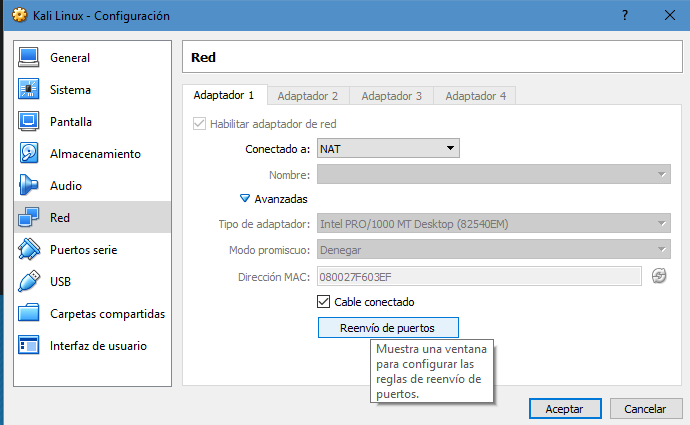
\includegraphics[width=1\textwidth]{04-REENVIOPUERTOS}
\end{figure}

Por \'ultimo agregamos una regla con los datos como se muestra a continuaci\'on: 

%Imagen 5
\begin{figure}[H]
\centering
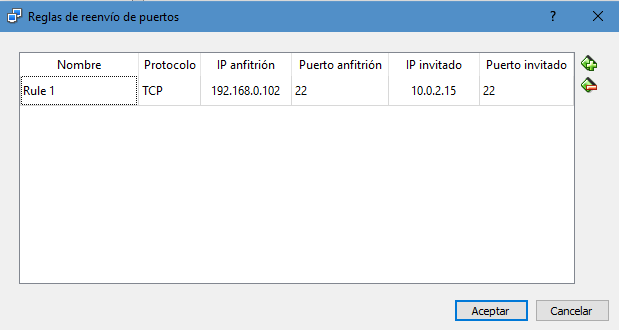
\includegraphics[width=1\textwidth]{05-CONFIGURADO}
\end{figure}

\subsubsection{Configuraci\'on servidor SSH en Kali linux}

En la terminal de Kali editamos del archivo \emph{/etc/ssh/sshd\_config} la l\'inea \emph{PermitRootLogin} y cambiamos su valor a \emph{yes}

%Imagen 6
\begin{figure}[H]
\centering
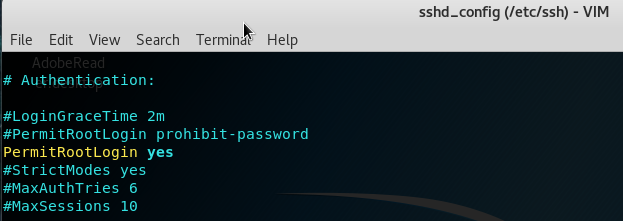
\includegraphics[width=1\textwidth]{06-CONFIGURACIONSSHD}
\end{figure}

Por \'ultimo inicializamos el servicio ssh, para ello tecleamos en la terminal \emph{/etc/init.d/ssh start}

%Imagen 7
\begin{figure}[H]
\centering
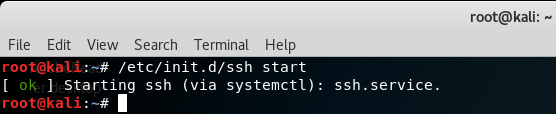
\includegraphics[width=1\textwidth]{07-STARTSSHD}
\end{figure}

Ya tenemos el servidor SSH listo para que accedamos desde Putty.

\subsubsection{Configuraci\'on de tunel SSH con Putty}

Abrimos Putty y tecleamos la IP a la que queremos conectarnos y dejamos el puerto estandar de ssh que es el 22 (ya configuramos virtualbox para que redirija las peticiones del puerto 22 a la m\'aquina virtual). Una vez ingresado la IP y el puerto, guardamos la sesi\'on.

%Imagen 8
\begin{figure}[H]
\centering
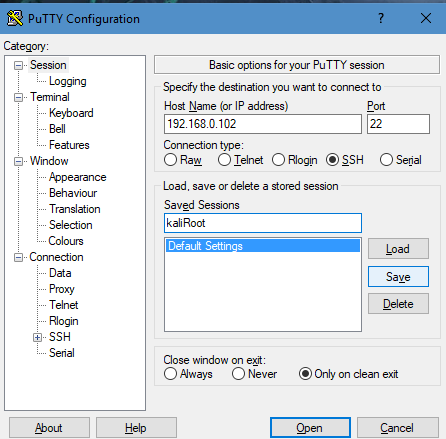
\includegraphics[width=1\textwidth]{08-GUARDARKALIPUTTY}
\end{figure}

Hacemos una prueba para ver que el servidor SSH de la m\'aquina virtual funciona correctamente, nos conectamos y nos logeamos con nuestras credenciales.

%Imagen 9
\begin{figure}[H]
\centering
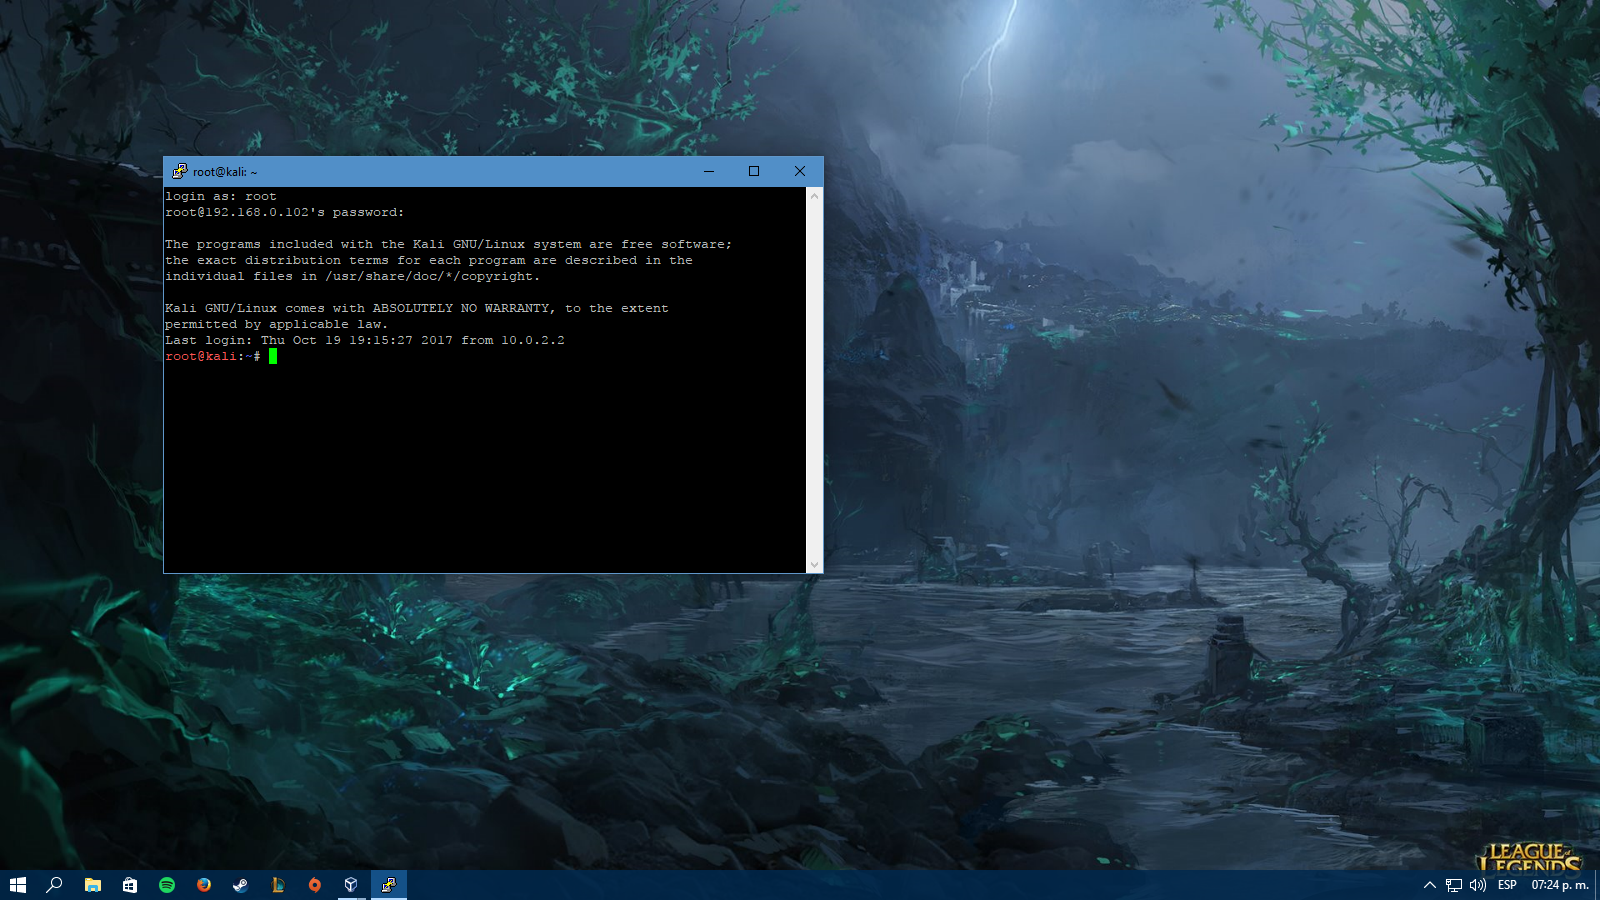
\includegraphics[width=1\textwidth]{09-LOGEADOSSH}
\end{figure}

Ya que pudimos acceder a la m\'aquina virtual por medio de SSH, ahora cargamos la sesi\'on que guardamos previamente y nos vamos al apartado \emph{Conection/SSH/Tunnels} en Putty. Ah\'i agregamos un puerto, en nuestro caso utilizamos el puerto \emph{50000}, marcamos la opcion \emph{Dynamic},le damos clic al bot\'on \emph{Add} y por \'ultimo nos conectamos de igual manera al paso anterior.

%Imagen 10
\begin{figure}[H]
\centering
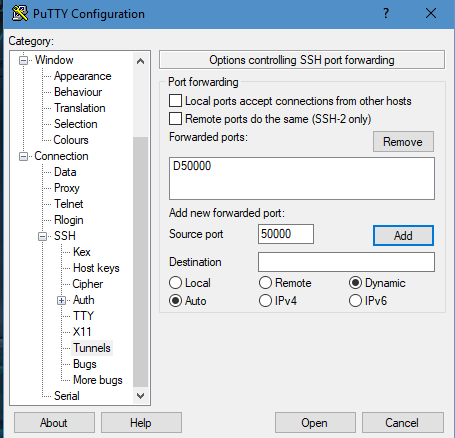
\includegraphics[width=1\textwidth]{10-PUERTO50000}
\end{figure}

\subsubsection{Configuraci\'on de Firefox}

Despu\'ues de preparar el tunel SSH, tenemos que configurar nuestro navegador para redirigir el tr\'afico a trav\'es del tunel. Para lo anterior nos vamos a las opciones de Firefox

%Imagen 11
\begin{figure}[H]
\centering
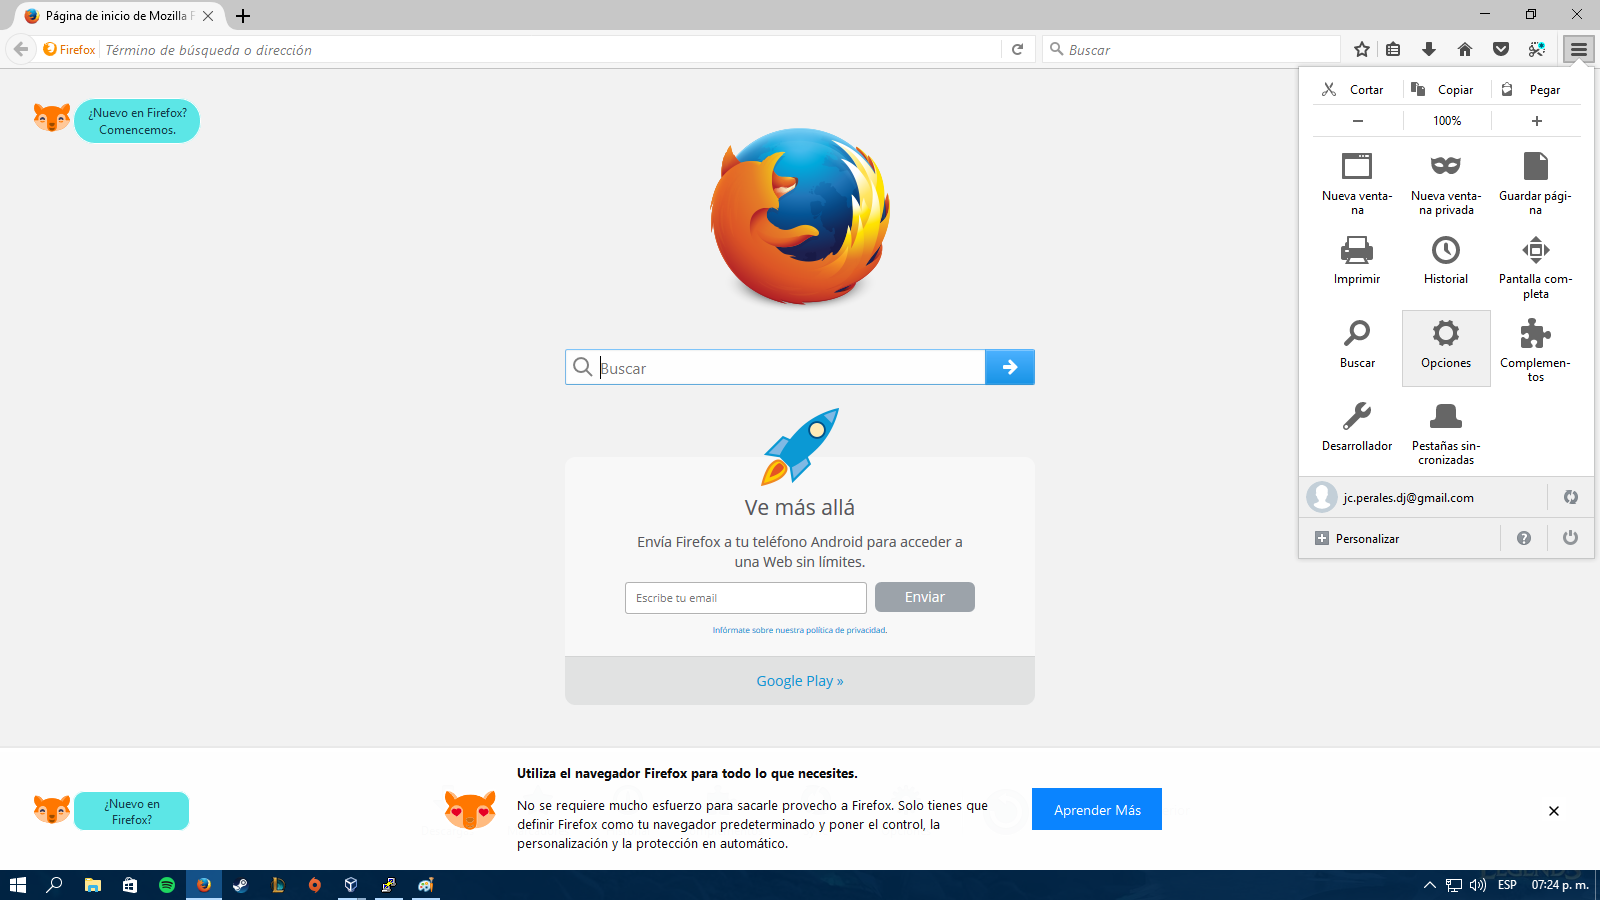
\includegraphics[width=1\textwidth]{11-OPCIONESFIREFOX}
\end{figure}

En la pestaña general, nos vamos a la secci\'on que dice \emph{Proxy de red} y damos clic en el bot\'on \emph{Configurar...}

%Imagen 12
\begin{figure}[H]
\centering
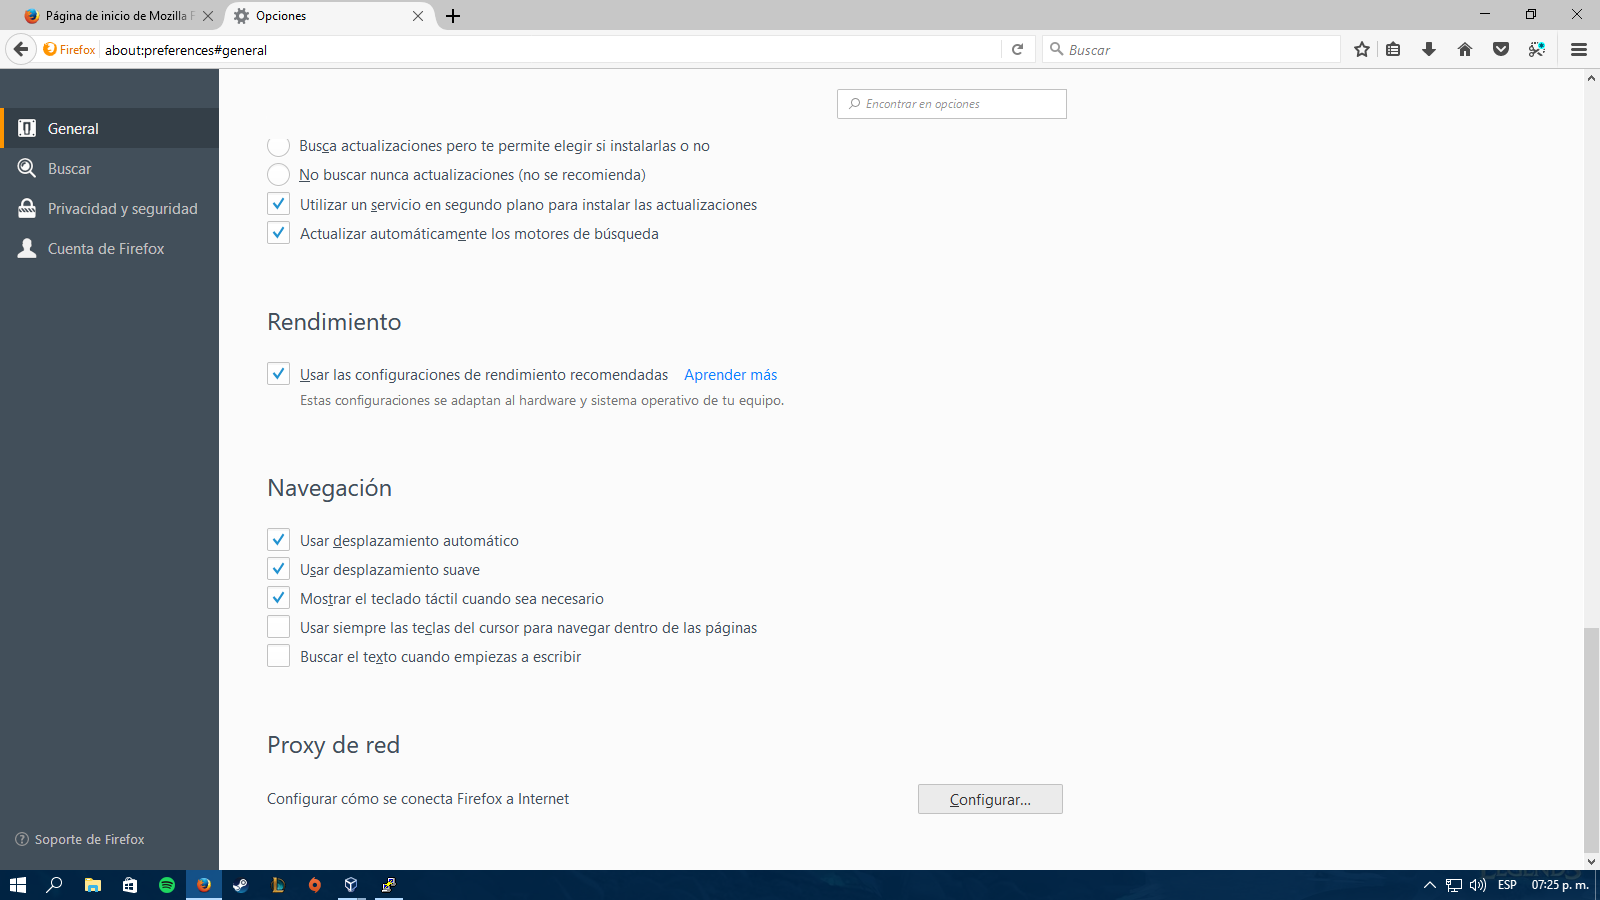
\includegraphics[width=1\textwidth]{12-CONFIGURACIONPROXY}
\end{figure}

Por \'ultimo marcamos la casilla que dice \emph{Configuraci\'on manual del proxy:} y en el cuadro de texto que dice \emph{Servidor SOCKS} ingresamos la IP \emph{127.0.0.1} (direcci\'on loopback) y en puerto asignamos el mismo que configuramos en Putty, es decir el \emph{50000}. 

%Imagen 13
\begin{figure}[H]
\centering
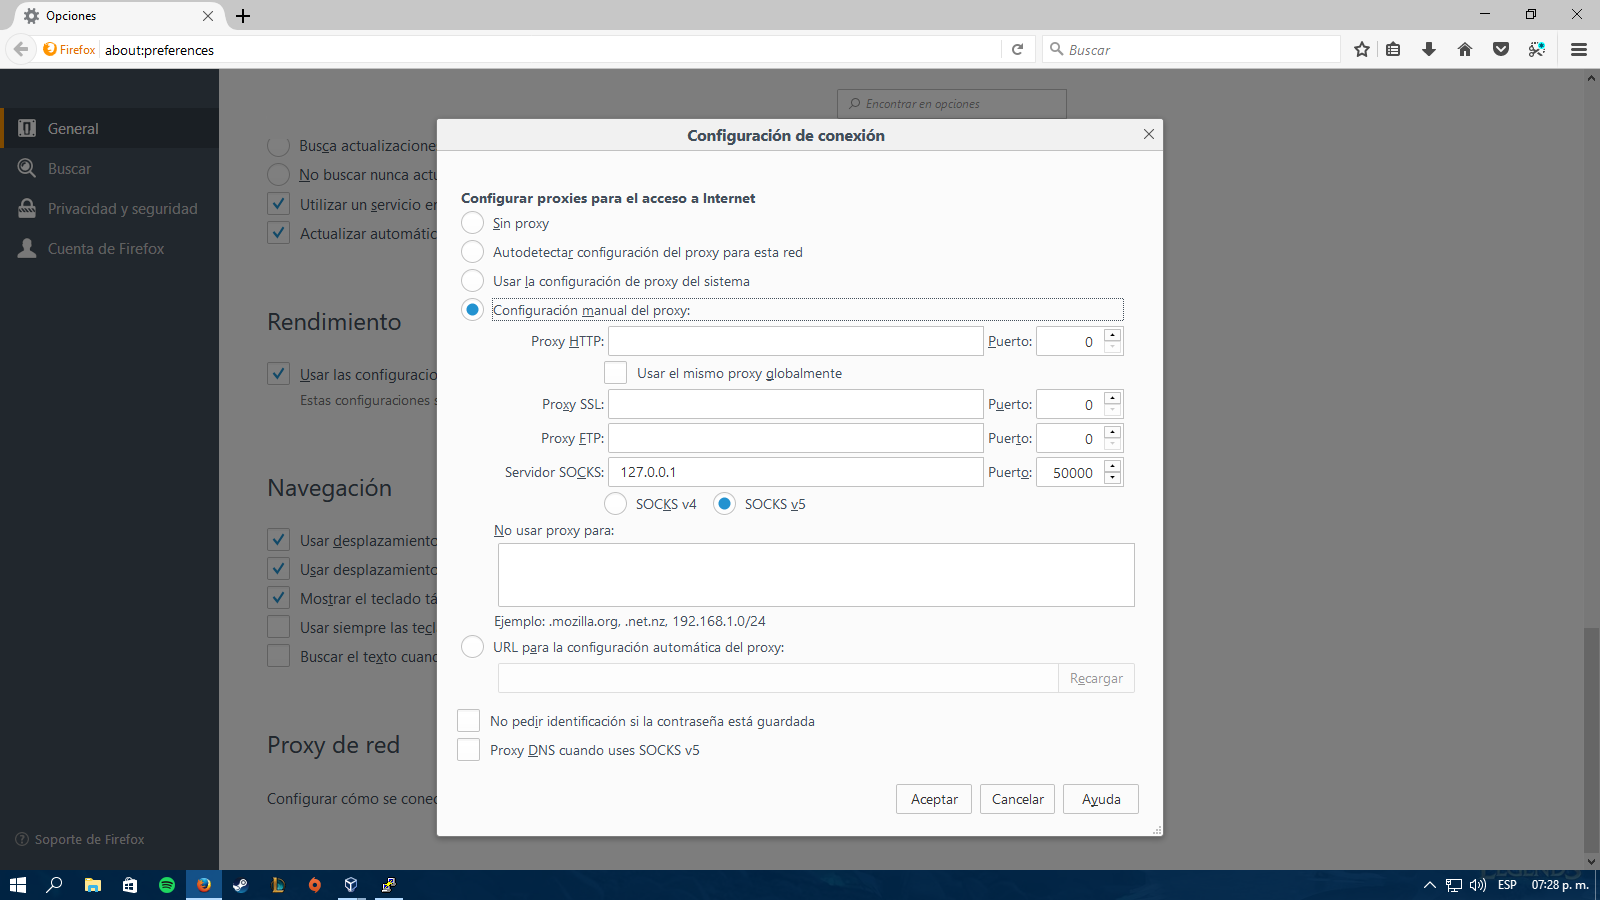
\includegraphics[width=1\textwidth]{13-CONFIGURACIONSOCKS}
\end{figure}

Damos clic en \emph{Aceptar} y listo, tenemos nuestro tunel SSH que pasa todo el tr\'afico enviado por Firefox en la m\'aquina host a la m\'aquina virtual kali linux de manera encriptada.

\section{Resultados}
\subsection{ARP Spoofing}
\subsection{Resultados del tunel SSH}
Para corroborar que funciona el tunel SSH, accedemos a una p\'agina sin seguridad, en este caso utilizamos \emph{www.gusanito.com}.

%Imagen 14
\begin{figure}[H]
\centering
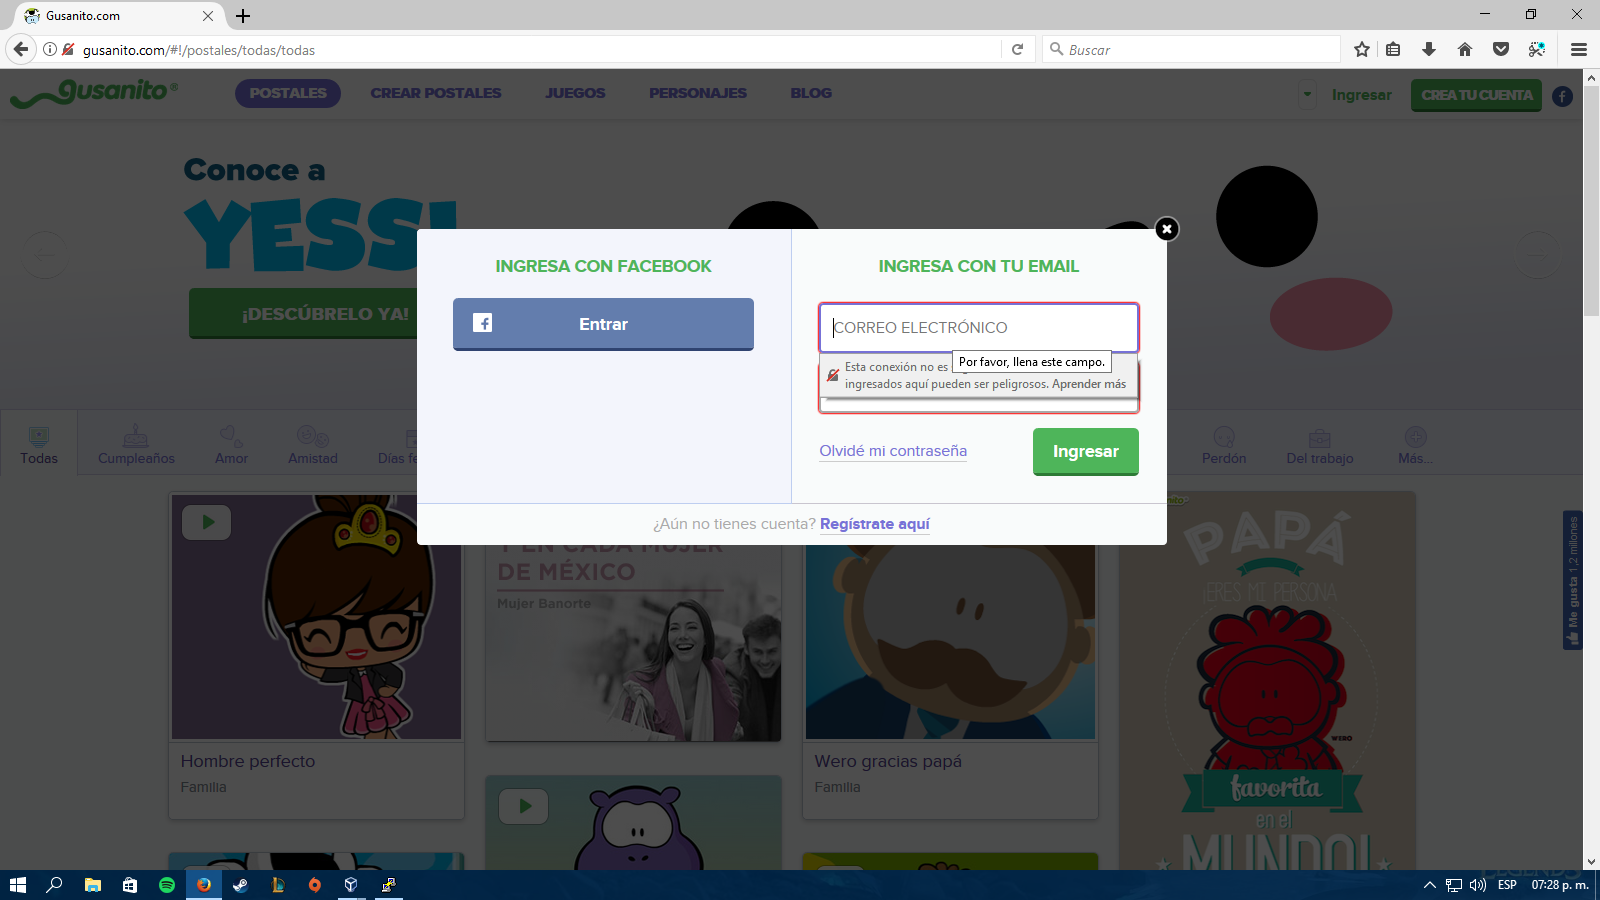
\includegraphics[width=1\textwidth]{14-GUSANITO}
\end{figure}

Ingresamos datos falsos para intentar acceder y antes de enviarlos, comenzamos a capturar los paquetes con Wireshark desde la m\'aquina virtual.

%Imagen 15
\begin{figure}[H]
\centering
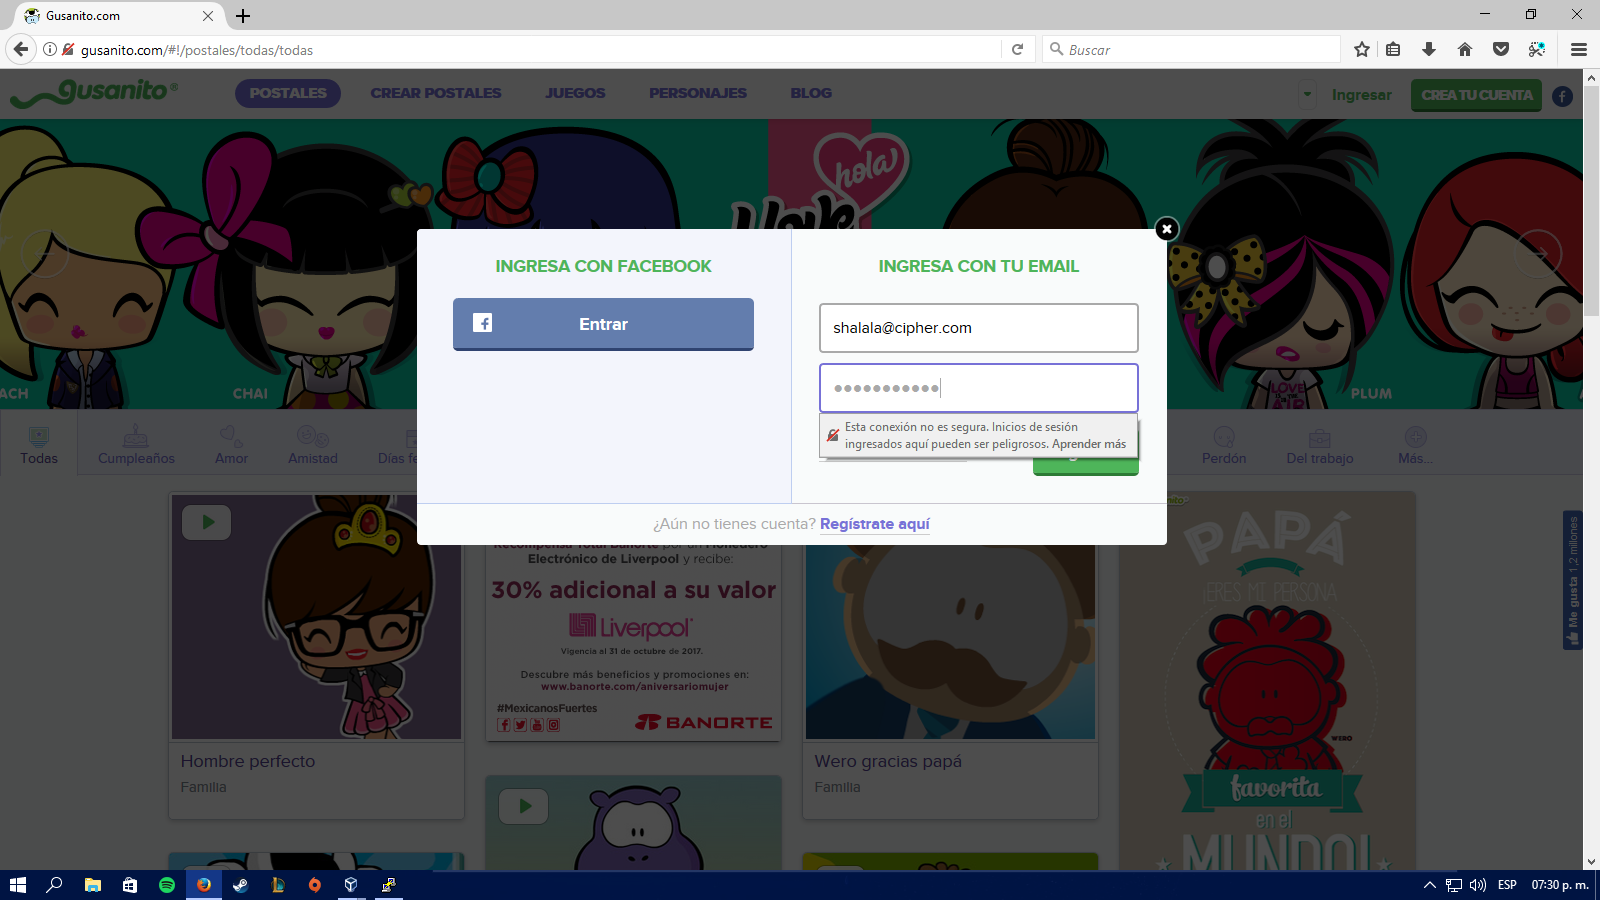
\includegraphics[width=1\textwidth]{15-CORREO}
\end{figure}

%Imagen 16
\begin{figure}[H]
\centering
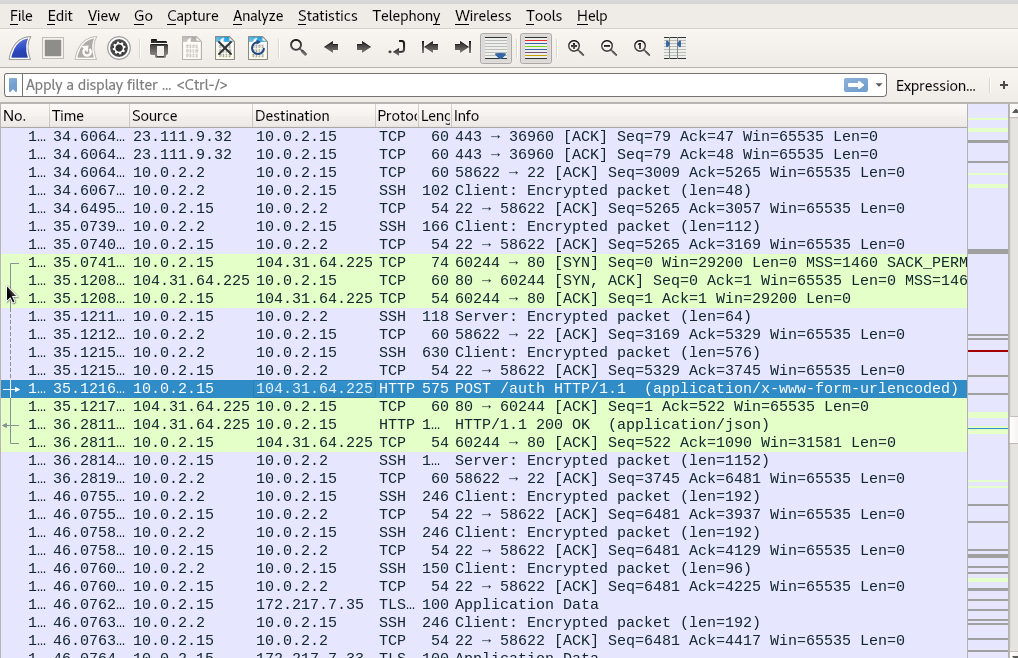
\includegraphics[width=1\textwidth]{16-WIRESHARKHTTPAUTH}
\end{figure}
Como podemos observar Wireshark captura muchos paquetes con el protocolo SSH los cuales van encriptados, sin embargo kali tiene que desencriptarlos para enviar las peticiones al servidor, por ello vemos un paquete HTTP AUTH, el cual se envia desde kali al servidor y no desde nuestro host.

Al final de lado de la m\'aquina remota, se siguen enviando los paquetes en claro.

%Imagen 17
\begin{figure}[H]
\centering
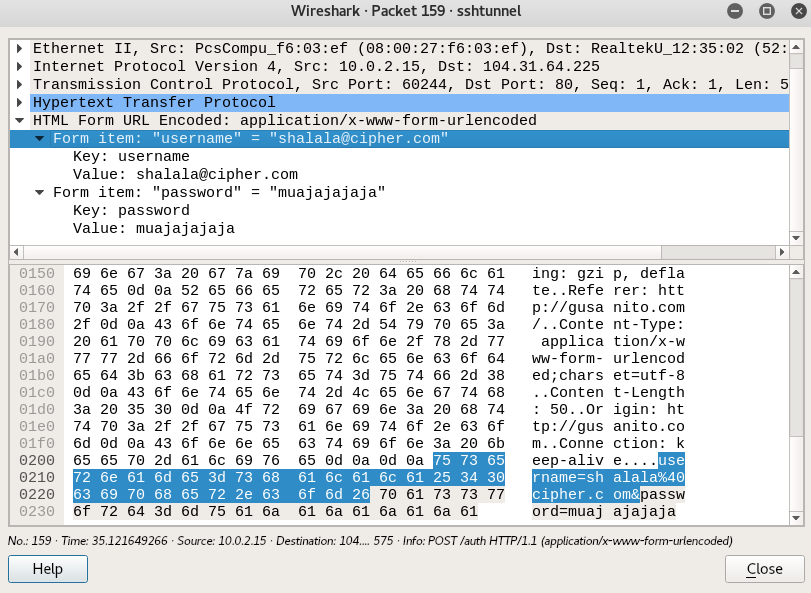
\includegraphics[width=1\textwidth]{17-CONTRASENAENCLARO}
\end{figure}

\section{Discusi\'on}

\subsection{ARP Spoofing}

\subsection{Tunel SSH}

Un tunel SSH sirve muy bien cuando en nuestra red, llamemosla 'A', tenemos incertidumbre sobre la seguridad de posible sniffering, de modo que nos conectamos a una red 'B' m\'as segura, para enviar todo el tr\'afico a trav\'es de la red B y no de la nuestra, la A, ya que si hay alguien escuchando en la red A, no podr\'a descifrar el contenido que viaja pues va encriptado en el tunel SSH.

\section{Conclusiones}
En la practica nos damos cuenta la falta de seguridad, para que no puedan interceptar nuestro trafico facilmente, por medio de sniffer como wireshark, 
si un atacante lanza el ataque hombre de enmedio estará interceptando la totalidad de nuestro tráfico tanto de entrada como de salida. como se vio se utiliz putty, con la ayuda del túnel SSH estaremos cifrando la totalidad de nuestro tráfico.

\section{Bibliograf\'ia}

\end{document}
